% This is LLNCS.DEM the demonstration file of
% the LaTeX macro package from Springer-Verlag
% for Lecture Notes in Computer Science,
% version 2.4 for LaTeX2e as of 16. April 2010
%
\documentclass{llncs}
%
\usepackage{makeidx}  % allows for indexgeneration
%
\usepackage{graphicx}
\usepackage{tabularx}
\usepackage{amssymb}
\usepackage{color}
\usepackage{upgreek}
\usepackage{listings}
%\usepackage{ tipa }
%\usepackage{relsize}
%\usepackage{caption}
%\usepackage{subcaption}
%\usepackage{multirow}
 \usepackage[table]{xcolor}
\definecolor{lgray}{gray}{0.6}
\definecolor{llgray}{gray}{0.75}
\definecolor{lllgray}{gray}{0.95}

\definecolor{dkgreen}{rgb}{0,0.6,0}
\definecolor{gray}{rgb}{0.5,0.5,0.5}
\definecolor{pink}{rgb}{1,0.07,0.57}

\lstset{frame=tb,
  language=Java,
  aboveskip=3mm,
  belowskip=3mm,
  showstringspaces=false,
  columns=flexible,
  basicstyle={\small\ttfamily},
  numbers=none,
  numberstyle=\tiny\color{blue},
  keywordstyle=\color{pink},
  commentstyle=\color{dkgreen},
  stringstyle=\color{blue},
  breaklines=true,
  breakatwhitespace=true
  tabsize=3
}

\graphicspath{{Bilder/}}
\hyphenation{
}
\usepackage[utf8]{inputenc}
\begin{document}

\title{Secure Coding: Phase 4 Report}

\author{Elias Tatros\\\email{elias.tatros@cs.tum.edu}\\}

\institute{Chair XXII Software Engineering\\Department of Computer Science, Technische Universität München}

\maketitle

%
\begin{abstract}
short description/overview
\keywords{Secure Coding, ASLR, CWE-329}
\end{abstract}
%
\section{Executive Summary}
%


\subsubsection{About the structure of this report\\}
Short overview over the structure of contents
%

\subsection{CWE-329: Use of static IV with Rijndael CBC}

Next9 bank makes use of a 512 bit hash value $scs_{seed}$. This value is used to generate TANs for the smart card simulator. It is recalculated after each successful transaction. The $scs_{seed}$ is generated on the server side and then encrypted using the Rijndael algorithm with a block size of 128 bits and a 128 bit key $k_{enc}$ (according to the AES-128 standard): $$enc_{k_{enc}} (scs_{seed}).$$
The encrypted 512 bit hash is saved to a file, which is then offered to the user for download. 

The user is supposed to download the file and use it as input for the smart card simulator, which in turn uses it to generate a TAN, that can be used to commit transactions. The user is asked to enter his 6 digit SCS PIN, which is utilized by the SCS to generate the decryption key $k_{dec}$. The key is then used to decrypt the 512 bit hash provided by the user. The original $scs_{seed}$ is obtained if $k_{enc} = k_{dec}$.

By inspecting the decompiled java code (and the php source code) we discovered, that a \emph{static IV} is used to initialize the cipher for \emph{CBC} (\emph{Cipher-Block-Chaining}) mode.
\begin{center}
\begin{figure}[hbtp]
        \centering
        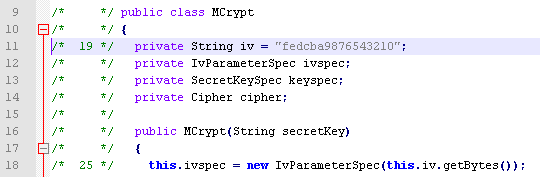
\includegraphics[natwidth=162bp,natheight=227bp]{staticIV.png}
        \caption{Use of static IV in CBC mode}\label{figStaticIV}
\end{figure}
\end{center}

Figure \ref{figStaticIV} shows an excerpt of the decompiled java code. It is notable, that the \emph{IV} is always initialized with the character sequence \emph{fedcba9876543210}. Using a static \emph{IV} in \emph{CBC} mode is a bad idea and a potential security weakness. In \emph{CBC} the plaintext is split into 16-byte blocks. Before encryption, each block is \emph{XORed} with the ciphertext of the previous block. This is true for all blocks, except for the first block, since there exists no ``previous ciphertext'' block to XOR it with. Because of this, the \emph{IV} is used as a substitude, effectively acting as the ciphertext of the ``-1'' block.

Using a static \emph{IV} with \emph{CBC} means that if two messages start with the same bytes, the ciphertext will be identical for the first (or even more) block(s). This gives unnecessary information to a potential attacker and can enable certain attacks. For example, if only a couple of short messages are sent (e.g. commands), which differ only in a few bytes (e.g. \emph{command=OPEN} vs. \emph{command=CLOSE}), an attacker can potentially determine which message carries what command by analyzing the frequency of each first block. 

It also completeley defeats the purpose of using an \emph{IV} with chaining mode at all, since an \emph{IV} in chaining mode is supposed to randomize the input of the first block, in the same way as it is done by \emph{CBC} for the following blocks.

A further problem is that the java code is run on client machines and accessible for any attacker that manages to decompile the jar file, which should be an easy task. It is therefore easy for an attacker to find the concrete value of the \emph{IV}. This value is not only valid for his machine and one message, but for all machines of all customers and for all messages. As shown in section \ref{SecMemoryScanAttack} this knowledge can be used to target customers with exploits that steal sensitive information, such as their SCS Pin and SmartCards.

\subsubsection{Change Recommendations}
The obvious solution is to use a different, randomly generated \emph{IV} for each encrypted message. It easily solves all of the problems mentioned. With a random \emph{IV} first blocks of ciphertexts are no longer identical even for identical plaintexts and attackers who decompile the jar can no longer gain easy access to a concrete \emph{IV} value, which prevents certain attacks, such as the one shown in \ref{SecMemoryScanAttack}. PHP \ref{listing:phpiv} and Java \ref{listing:javaiv} both offer functions to create cryptographically secure random initialization vectors, as shown below.

\begin{lstlisting}[caption= PHP IV generation,label=listing:phpiv]
 $iv_size = mcrypt_get_iv_size(MCRYPT_RIJNDAEL_128, MCRYPT_MODE_CBC);
 $iv = mcrypt_create_iv($iv_size, MCRYPT_RAND);
\end{lstlisting}

\begin{lstlisting}[caption= Java IV generation,label=listing:javaiv]
SecureRandom random = new SecureRandom();
byte iv[] = new byte[16];
random.nextBytes(iv);
IvParameterSpec ivspec = new IvParameterSpec(iv);
\end{lstlisting}

\subsection{Weakness in key generation and padding}
The effectiveness of a symmetric encryption algorithm in terms of the provided confidentiality is always depended on the key size. An advanced encryption standard, such as AES is not a silver bullet. The security of symmetric encryption algorithms is quickly compromised if configured with insufficient care.


The next9 bank encryption key is generated by taking the users SCS password (a $6$ character number) and then padding it with the character sequence ``0000000000''. The key is not derived from the password in any way, but rather the key is the actual password plus $80$ bits of $0$ padding. Therefore the meaningful bits of the key are reduced to the size of the password, which is $6$ characters or $48$ bits long. Even if all bits were perfectly random and uniformly distributed, we would already consider this to be a pretty weak key.

However, we also know that the SCS password can only consists of digits, which drastically reduces the entropy of the key even further. A 48 bit key can result in $2^{48}$ different values. When doing encryption it is important that every single one of these values has the same probabilty of ocurrence. This is what CSPRNGs (cryptographically secure pseudo-random number generator) are usually used for.  In the optimal case a 48 bit key produced by a CSPRNG would have an entropy of 48 bits.

However, in this case the bits in the key are not uniformly distributed. In fact, for a 6 digit number each digit can take on a value between $0$ to $10$, resulting in a total of $10^6$ or $1$ million values. Such a string gives $20$ bits of entropy in the best case, meaning if we assume that each digit in the SCS password is chosen completeley randomly. 

The method of key generation used significantly reduces the strength of the key and consequently the effectiveness of the entire encryption. A $48$ bit key with only $20$ bits of entropy does not measure up to todays encryption standards. 

\subsubsection{Change Recommendations}
A quick fix for this issue would be to remove the 0 padding and generate the key by running the SCS password through a cryptographic hash function, such as HMAC. In a final step the output would be reduced to the first $128$ bits, resulting in a more secure key.

\subsection{Memory Scan Attack}
\label{SecMemoryScanAttack}
After gaining knowledge of the weaknesses in the encryption module we developed a method to exploit the usage of the static \emph{IV} and the flawed key generation technique.

\subsubsection{Client Side Analysis}
Our attack is aimed at the client machines of customers using the smart card banking method provided by Next9. The attack shows that a large amount of sensitive data is stored in memory for long times. The data is stored in plain text, not encrypted or hashed. This includes the users SCS Pin, the seed (which effectively acts as the smart card) in encrypted and unencrypted form and the symmetric encryption key. Once an attacker obtains the seed and the pin, he can create his own smart card from the seed and use the pin to commit his own transactions on behalf of the user.
\begin{center}
\begin{figure}[hbtp]
        \centering
        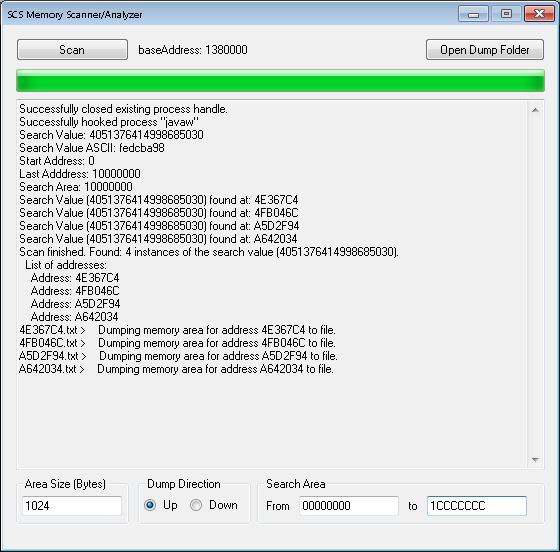
\includegraphics[scale=0.6]{Scanner.png}
        \caption{Our SCS Memory Scanner}\label{figMemoryScanner}
\end{figure}
\end{center}
During our analysis we wrote a custom program, which is able to obtain the sensitive data from memory using the static \emph{IV} (fedcba9876543210) as a ``point of reference''. The \emph{IV} was discovered within the decompiled SCS jar. For experimentation and demonstration purposes the program comes with a usable GUI, as shown in Figure \ref{figMemoryScanner}. An actual exploit would of course be deployed invisibly (for example via some drive-by download, USB stick, etc.) or hidden as a trojan in a seemingly useful user application.

The scanner works by opening the java process executing the SCS module and obtaining its memory base address. Since the SCS program stores sensitive data as plaintext in strings it is quite easy to find occurrences of this data in memory. In the scan step the program searches for a byte sequence which is equal to the static \emph{IV}. The search process can be limited to a memory offset area (from the base address) specified under ``search area'', which can speed up the task in some cases. Usually the scanner will find 6 instances of the plaintext static \emph{IV} in memory and ``remember'' those specific addresses.
\begin{center}
\begin{figure}[hbtp]
        \centering
        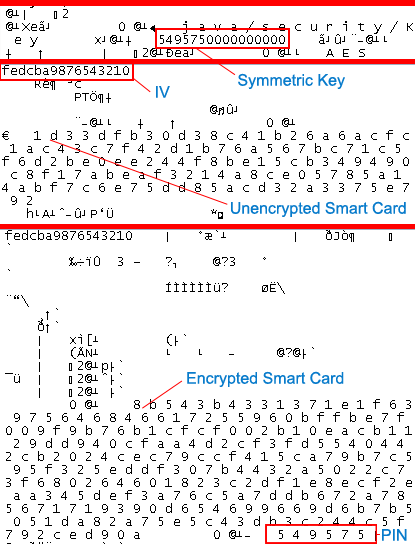
\includegraphics[scale=0.6]{dump.png}
        \caption{Sensitive Information in plain text}\label{figDump}
\end{figure}
\end{center}
By dumping the memory around these addresses we can find other sensitive data, which includes the users SCS PIN, the seed (unencrypted and encrypted) and the encryption key in plain text. The program enables us to dump memory located below and above the addresses of interest and we can also specify the size of the dump in bytes. Figure \ref{figDump} was constructed from 3 different dump files (divided by red bars), each containing 1024 bytes of data around three of the six addresses of interest (static \emph{IV} locations). One can easily make out the sensitive data and automatically parse it. Given the knowledge that the encryption key is made up by the user pin and 10 zeros of padding we can immediately locate the user pin and encryption key. We can identify which of the two seeds is the ciphertext or plaintext by applying the encryption key in combination with the \emph{IV} to each sequence. If we obtain one of the sequences by encrypting the other, we found the unencrypted seed.
An attacker could modify the program to automatically send those dumps to some collecting machine over the network. After obtaining the user pin and smart card (seed), he or she is able to commit transactions on behalf of that user to any destination, simply by downloading the SCS Software from the Next9 website, pasting one of the seeds into a file (smart card), loading this file in the SCS and entering the corresponding user pin.

\subsubsection{Server Side Analysis}
Server side Next9 bank does a good job of keeping attackers at bay. We did not find any practical attacks that could be used to exploit the encryption weaknesses on the server side. From our point of view the only potential attack surface presented on the server side is the C program for batch transaction processing. The C program was decompiled without issues and it seems that no code obfuscation was used. We did not find any way to directly cause stack overflows or similar vulnerabilities through the manipulation of program input. However, the C program is definiteley susceptible to memory tampering attacks. 

There is seemingly no protection versus memory tampering and the simple structure of the program makes it easy to find static pointers to sensitive data such as user TANs used in transactions. Given a static pointer not even a scanner would be required. Using mostly the same techniques as done in our memory scan attack for the client SCS program, a similar attack can be mounted against the server side batch transaction parser program. For example, a hidden program could be used to attach to the parser process, reading the sensitive data from memory and sending it over the network to the attacker. Although, we do admit that deploying such a program would not be an easy task, since one would first require access to the machine which is running the parser program. It is however still a possibility that someone with sufficient access could be able to deploy the exploiting program, for example via a USB stick or possibly some remote access software used in server administration. Also the discovery of some future loophole might enable attackers to deploy the program without insider help.

\subsubsection{Change Recommendations}
We recommend the usage of address space layout randomization (ASLR) and pointer encryption for both the server side parser and the client side SCS program. While ASLR is active on the linux VM, this only randomizes the locations of stack and libc addresses. In order to create a truly position independent executable it is necessary to use the compiler flag \emph{-PIE}. On gcc the relevant flag is \emph{-fPIE}. Tools such as PointGuard can prevent pointer corruption and many related attacks by encrypting pointers and only decrypting them when loaded into CPU registers.

For java we recommend that any information that needs to be stored persistently is encrypted in memory. Any confidential information that can not be encrypted should quickly be purged from memory after use. This means that Strings can not be used to store sensitive data such as initialization vectors, user PINs or encrytpion keys. This is because Strings are immutable and can not safely be overwritten in memory. Instead one should use StringBuilder or an array of characters, or a custom data structure. A better approach might be to directly access memory via unsafe code to store sensitive data and then erase its contents after processing. This technique is described in the Oracle java secure coding guidelines under \emph{Guideline 2-3 / Confidential-3}. Additionally, we recommend turning off core-dumps as these can leak sensitive data that was in memory. As a last step it might be a good idea to digitally sign the jar file, which could prevent the distribution of tampered SCS jars.

\subsection{C \& Java Program Decompilation}

\subsection{PHP \& JavaScript Code Review}
- PHPSecAudit: no luck\\
- RATS: didn't get it to work\\
- RIPS: found a few false positives, maybe 1 of interest, see screenshots\\
%
% ---- Bibliography ----
\end{document}
